\section{Espacio de datos}

Los espacios de datos son contenedores que aíslan las diferentes versiones de la información de los conjuntos de datos. Para el caso del área de finanzas se han construido los siguientes espacios de datos “dataspaces”:

\begin{enumerate}
    \item [CA] Catálogos Maestros. Espacio que aloja los catálogos maestros dentro de CMI. 
    \item 
    \item [CuCo] Cuentas Contables – Landing V2.  Espacio de aterrizaje de los datos. 
    
    \item [CuCo] Cuentas Contables V2. Espacio que contiene los datos relevantes en las Cuentas Contables.
    
    \item [CuCo] Cuentas Contables – Calidad V2.  Espacio para aplicar las reglas de calidad. 
    
    \item [CA] Customized Administration. Espacio donde se configuran las solicitudes para proceso de integración.
    
    \item Historico. Espacio donde se aloja el historial de los datos, además de contener el proceso de aprobación masiva dado el caso. 

\end{enumerate}


\section{Reglas de Calidad}

En este apartado, se describen de manera funcional las reglas de calidad para el proceso de Cuentas Contables, las cuales se trabajaron con el equipo funcional de CMI. Éstas son:

\begin{itemize}
    \item \textbf{Correcta longitud y formato de una cuenta contable}
    
    Una cuenta contable debe tener una cierta longitud y cierto formato para considerarse como una, por lo que se valida estos casos.
    \item \textbf{Descripciones de cunetas contables validas}
    
    Se verifica que dentro el campo solo se encuentren cadenas de texto.
    \item \textbf{Existencia de cuentas 49}
    
    Se verifica si una cuenta contable inicia con los valores de 4 a 9.
    \item \textbf{Existencia de cuentas 1-3}

    Se verifica si una cuenta contable inicia con los valores de 1 a 3.
    \item \textbf{Completitud en campos}
    
    Se verifica que los campos especificados no sean vacíos.
    \item \textbf{Cuentas Activas}
    
    Se verifica las banderas respectivas se encuentren desactivadas para considerar una cuenta activa.

\end{itemize}

\section{Perspectivas de datos}

La perspectiva está asignada por roles o usuarios y solo estos pueden tener acceso y visibilidad de ella.

\begin{figure}[H]
    \centering
    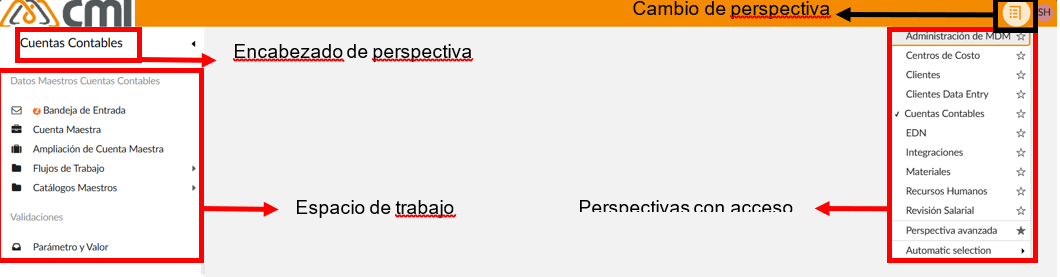
\includegraphics[width=0.8\textwidth]{EspacioReglasPerspectiva/ImgPerspectiva/PD01.png}
    \caption{Ejemplo de perspectiva de CuCo}
\end{figure}

Para cambiar de perspectiva, es necesario seleccionar el acceso a perspectivas activas, que despliega una lista de las disponibles para el usuario. Al hacer clic en una de ellas, se redirige automáticamente a la perspectiva elegida.

\begin{enumerate}
    \item Perspectiva de CuCo V2 ([FIN] Cuentas Contables V2) 
    
    Esta perspectiva consta de los siguientes elementos:

    \begin{enumerate}
        \item Bandeja de entrada: Tareas de usuario activas que requiere la participación de éste o uno del mismo rol.
        \item Cuenta Maestra: Tabla con información referente a las cuentas contables.
        \item Ampliación de Cuenta Maestra: Tabla con información referente a las cuentas contables que fueron ampliadas.
        \item Flujos de Trabajo
        \begin{itemize}
            \item Flujos de Trabajo: Vista de flujos de trabajo pertenecientes al proceso.
            \item Flujos de Trabajo Activos: Flujos de trabajo que se encuentran ejecutándose.
            \item lujos de Trabajo Completos: Flujos de trabajo que completaron su proceso. 
        \end{itemize}
        \item Catálogos Maestros
        \begin{itemize}
            \item Mandante: Tabla de información perteneciente a Catálogos Maestros referente a la información del mandante.
            \item Nivel 1: Catalogo funcional que contiene la información del primer nivel de una cuenta contable, este catálogo depende del tipo de Banco.
            \item Nivel 2: Catalogo funcional que contiene la información del segundo nivel de una cuenta contable, este espacio depende del primer nivel. 
            \item Nivel 3: Catalogo funcional que contiene la información del tercer nivel de una cuenta contable, este espacio depende del segundo nivel.
            \item Nivel 4: Catalogo funcional que contiene la información del cuarto nivel de una cuenta contable, este espacio depende del tercer nivel.
            \item Nivel 5: Catalogo funcional que contiene la información del quinto nivel de una cuenta contable, este espacio depende del cuarto nivel.
            \item Nivel 6: Catalogo funcional que contiene la información del sexto nivel de una cuenta contable, este espacio depende del quinto nivel además de contener la descripción de la cuenta y cuenta alternativa.
        \end{itemize}
        \item Historico
        \begin{itemize}
            \item Cuenta Contable Ampliación/Multi sociedad: Contiene el historico de operaciones donde se usan varias sociedades.
            \item Cuenta Contable PUC: Contiene el historico de operaciones a nivel PUC creación/ modificación/ bloqueo/ desbloqueo.
            \item Cuenta Contable Multimandante: Contiene el historico de operaciones a nivel PUC creación/ modificación/ bloqueo/ desbloqueo a varios mandantes a la vez.
            \item Cuenta Contable Modificación/ bloqueo/ desbloqueo: Contiene el historico de operaciones a nivel sociedad enfocado en una sola sociedad a la vez.
            \item Cuenta Contable CUSA: Contiene el historico de operaciones relacionados al mandante CUSA.
        \end{itemize}
        \item Aprobaciones masivas
        \begin{itemize}
            \item Nivel PUC
            \begin{itemize}
                \item NEFI Aprobación Masiva: Vista para el proceso masivo enfocado en el validador NEFI.
                \item Datos Maestros Aprobación Masiva: Vista para el proceso masivo enfocado en el validador de Datos Maestros.
            \end{itemize}
            \item Nivel Sociedad
            \begin{itemize}
                \item NEFI Aprobación Masiva: Vista para el proceso masivo enfocado en el validador NEFI.
                \item Datos Maestros Aprobación Masiva: Vista para el proceso masivo enfocado en el validador de Datos Maestros.
            \end{itemize}
        \end{itemize}
        
        \item Parámetro y Valor Tabla de información perteneciente a Customized Administration
    \end{enumerate}

    \item Perspectiva Avanzada

    Al estar dentro de la herramienta se tiene una vista inicial donde se encuentran los apartados más relevantes del proceso de Cuentas Contables.
\end{enumerate}

\begin{figure}[H]
    \centering
    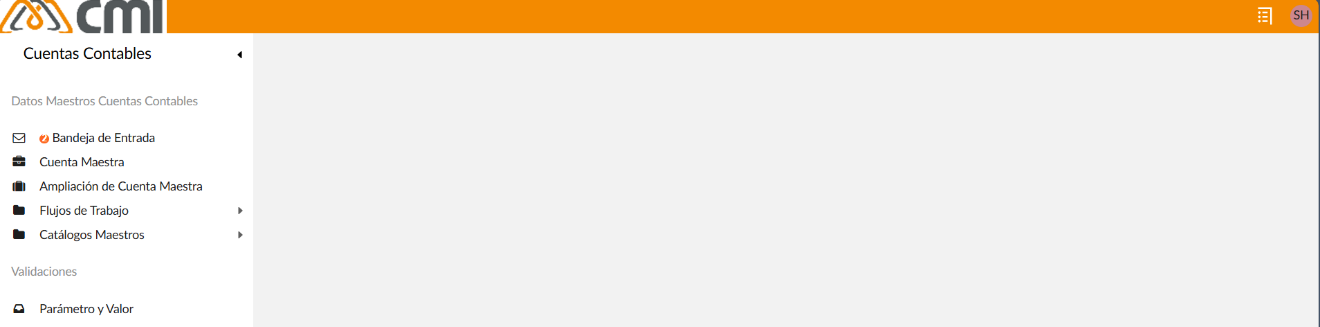
\includegraphics[width=0.8\textwidth]{EspacioReglasPerspectiva/ImgPerspectiva/PD02.png}
    \caption{Vista Inicial al acceder a TIBCO EBX}
\end{figure}

Si el usuario al cuenta con los permisos necesarios, al dar clic sobre el apartado de perspectivas, le permitirá ver el acceso a otras perspectivas. 
En este caso se hace referencia a la perspectiva avanzada, 
la cual tiene el nombre \textbf{“Advanced Perspective”} si se encuentra la herramienta en inglés; si se encuentra en español será “Perspectiva Avanzada”.

Al dar clic sobre este acceso se redirecciona a la vista de administrador. Se puede confirmar el acceso a este apartado al ver los íconos señalados en la siguiente imagen. 
Esta vista está disponible para los usuarios con permisos de administrador. 

\begin{figure}[H]
    \centering
    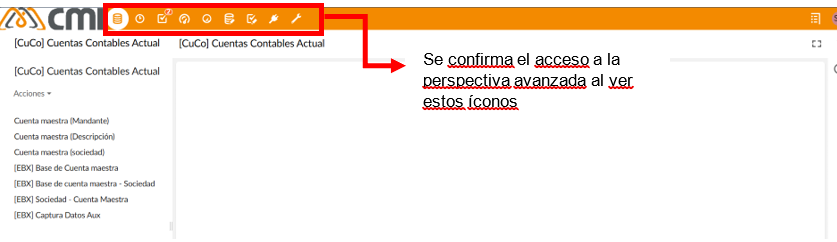
\includegraphics[width=0.8\textwidth]{EspacioReglasPerspectiva/ImgPerspectiva/PD03.png}
    \caption{Perspectiva Avanzada TIBCO EBX.}
\end{figure}
